\externaldocument{main.tex} 
Packaging an Electron application can be carried out in two different ways which each have multiple options.
The first way is to use tooling such as electron-forge. 
The options and details with this approach will be explained later in this chapter.
The other way is to not use any tools and create a distribution manually.\paragraph{}
This can either be done by downloading the prebuilt Electron binaries and copying the 
source code into the correct location or by packaging source code into a source code archive.
The source code archive approach is beneficial in that it improves performance of file reads
on Windows. 
However, both of these approaches require additional work after the fact such as branding. \parencite{electronDocsDist}\paragraph{}
To avoid these steps it is recommended to use one of the tools available which handle packaging
the application.
These tools include electron-forge, electron-builder and electron-packager with each of them
tasked with creating the same outcome but in different ways.
In this example the application will be built with electron-packager.\paragraph{}
As mentioned previously Electron Packager is a command line tool which handles packaging 
Electron source code for distribution. 
It supports all major platforms such as Windows, Linux and MacOS which makes it trivial
for developers to create a distribution for each target platform using just one tool. \parencite{electronPackager}\paragraph{}
Electron Packager can be installed via \acrshort{npm}.
\begin{lstlisting}[caption=Installing Electron Packager]
npm install --save-dev electron-packager
\end{lstlisting}
Note that according to the project documentation it is not recommended to install the module globally. \parencite{electronPackager}
After the installation process has finished one can start building the various distributions. 
As this project was developed on a Linux machine the first distribution to be created will be a \acrfull{deb}.
The first step is to set a product name property as Electron Packager looks for such a property in the package.json file.
\begin{lstlisting}[caption=Product name property in package.json]
{
  "name": "pze",
  "productName": "PZE",
}
\end{lstlisting}
After setting the product name one can begin to build the package.
\begin{lstlisting}[caption=Command for using Electron Packager]
electron-packager . <app-name> --overwrite --asar=true --platform=<target-platform>
--arch=<x64|x86> --icon=<path/to/icon> --prune=true --out=<path/to/outDir>
\end{lstlisting}
This is the basic command for creating a build. 
The following list describes the possible values for each parameter and their meaning:
\begin{itemize}
    \item \lstinline[columns=fixed]{<app-name>} The app name specified in package.json by the name field.
    \item \lstinline[columns=fixed]{--overwrite} Optional flag for overwriting any previously created distributions.
    \item \lstinline[columns=fixed]{--asar=true} Optional flag for using asar, which is an extensive archive format
    that concatenates all files without compression.
    \item \lstinline[columns=fixed]{--platforn} The platform to build for (Windows, Linux MacOS).
    \item \lstinline[columns=fixed]{--arch} A flag for the desired architecture. 
    Can be omitted together with --platform if the --all flag (creates bundles for all
    platforms and architectures).
    \item \lstinline[columns=fixed]{--icon} Optional flag for setting the application icon.
    \item \lstinline[columns=fixed]{--prune=true} Runs the npm-prune --production command to remove all developer dependencies
    from the project.
    \item \lstinline[columns=fixed]{--out} Flag to specify the output directory.
\end{itemize}
Of course, this command can also be specified in package.json:
\begin{lstlisting}[caption=Command for Linux build specified in package.json]
"package-linux": "electron-packager . pze --overwrite --asar=true --platform=linux --arch=x64 --prune=true --out=release-builds"
\end{lstlisting}
The above example is the command for creating a package for Linux with the x64 architecture.
Once this is defined one can create the build by running \lstinline[columns=fixed]{npm package-linux}.
This process can now be repeated for each other target platform, in this case Windows and MacOS. 
Note however that a MacOS distribution can only be signed when built on a MacOS platform. \parencite{electronDocsDist}
\begin{lstlisting}[caption=Commands for Windows and MacOs builds specified in package.json]
"package-mac": "electron-packager . pze --overwrite --platform=darwin --arch=x64 --prune=true --out=release-builds",
"package-win": "electron-packager . pze --overwrite --asar=true --platform=win32 --arch=ia32 --prune=true --out=release-builds --version-string.CompanyName=CommUnity --version-string.FileDescription=CommUnity --version-string.ProductName=\"PZE\"",
\end{lstlisting}
As seen above the windows build needs some additional parameters which define the company name and description. 
If those are not set the application will simply appear as "Electron" in Windows. \parencite{winElectronAppStr}\paragraph{}
After having packaged the application it is then time to create the installers. 
The first example will detail the creation of a \acrshort{deb} package. 
For this, the Electron Installer Debian is required. 
It can be installed via \acrshort{npm}:
\begin{lstlisting}[caption=Installation of electron-installer-debian]
npm install -g electron-installer-debian
\end{lstlisting}
Electron Installer Debian also requires a configuration in which certain details such as the
icon, destination and application categories. 
\begin{lstlisting}[caption=Configuration for debian package: debian.json]
{
    "dest": "release-builds/",
    "categories": [
        "Utility"
    ],
    "lintianOverrides": [
        "changelog-file-missing-in-native-package"
    ]
}
\end{lstlisting}
Optionally an icon can be specified, which has been omitted in this case. 
The categories field describes the type of the application such as game, science or in this case utility.
Lastly there is a property to quiet Lintian, which is a debian package checker.
The installer creation needs its own script with a few properties, which can be defined in 
package.json as well:
\begin{lstlisting}[caption=Configuration for debian package: debian.json]
"create-debian-installer": "electron-installer-debian --src release-builds/pze-linux-x64/ --arch amd64 --config debian.json"
\end{lstlisting}
The flags in this command have the following purpose:
\begin{itemize}
    \item \lstinline[columns=fixed]{src} Points to the location where the created installer should be saved.
    \item \lstinline[columns=fixed]{--arch} Defines the architecture.
    \item \lstinline[columns=fixed]{--config} Points to the required configuration file.
\end{itemize}
As the Electron Packager has already run one can now run Electron Debian Installer with 
\lstinline[columns=fixed]{npm run create-debian-installer}.
This will result in a \acrshort{deb} package which can be installed on Linux:
\begin{figure}[H]
    \centering
    \label{fig:pze-deb-package}
    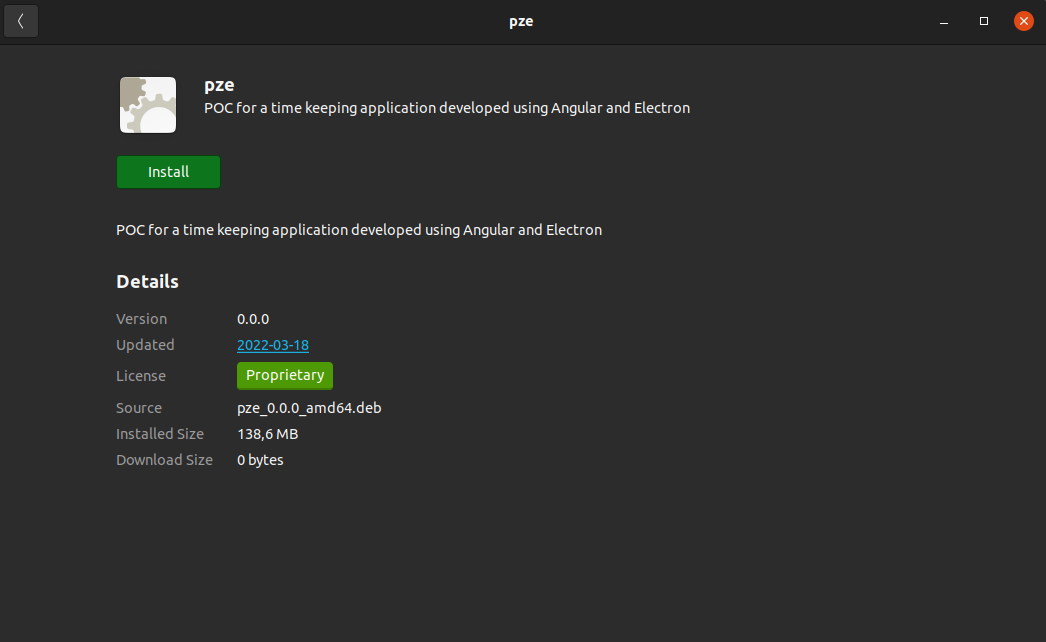
\includegraphics[width=0.8\textwidth]{deb-package}
    \caption{Installer for the recently created \acrshort{deb} package}
\end{figure}
